% coding:utf-8

%FOSASTOC, a LaTeX-Code for a electrical summary of stochastic
%Copyright (C) 2013, Daniel Winz, Ervin Mazlagic

%This program is free software; you can redistribute it and/or
%modify it under the terms of the GNU General Public License
%as published by the Free Software Foundation; either version 2
%of the License, or (at your option) any later version.

%This program is distributed in the hope that it will be useful,
%but WITHOUT ANY WARRANTY; without even the implied warranty of
%MERCHANTABILITY or FITNESS FOR A PARTICULAR PURPOSE.  See the
%GNU General Public License for more details.
%----------------------------------------

\chapter{Grundbegriffe}
\newpage

\setkeys{Gin}{width=1\textwidth}

\section{Arithmetisches Mittel}
Das \gls{arithmetische Mittel} beschreibt den Quotienten aus 
der Summe aller Elemente und der Anzhal Elemente. Dieses wird oft auch
einfach als Mittelwert, \gls{Mittel} oder \gls{Durchschnitt} bezeichnet. 
Ein solcher Mittelwert wird mit einem übergestellten Strich  
markiert.
$\bar{x}$.
\[ 
	\bar{x} 
	= \frac{1}{n} \cdot \left( \sum_{i=1}^{n} x_i \right)
	= \frac{x_1 + x_2 + \dots + x_n}{n}
\]
Ein allseits bekanntes Beispiel für das arithmetische Mittel ist der 
\emph{Notendurchschnitt}. 

\paragraph{Berechnung in R}
In \lstinline{R} wird das arithmetische Mittel mit der Funktion 
\lstinline{mean()} ermittelt.
\begin{Schunk}
\begin{Sinput}
> a <- c(6,4,5,5,4,5,6,3,4,5,6)
> mean(a)
\end{Sinput}
\begin{Soutput}
[1] 4.818182
\end{Soutput}
\end{Schunk}

\section{Quantil}
Ein \gls{Quantil} beschreibt eine Grenze innerhalb einer sortierten 
Datenreihe. Diese wird stets in Prozenten angegeben, d.h. 
\emph{5\% Qunatil, 20\% Quantil} usw. 
Beispielsweise ein 5\% Quantil ist eine Stelle in der Datenreihe, an 
welcher 5\% der Werte unterhalb dieser Grenze liegen (z.B. \emph{5\% 
aller E-Mails sind kürzer als 12 Worte $\Rightarrow$ 12 ist das 5\%
Quantil}).
\[ \begin{array}{l l}
	\alpha \in [0, 1] 
		& \text{Prozentwert der Grenze} \\
	x_1 - x_n
		& \text{Elemente sortiert nach grösse} \\
	\alpha \cdot n 
		& \text{Qunatil} \\
\end{array} \]
Bei der Berechnung des Quantils gilt es zu beachten ob die Elemente 
der Datenreihe ganze oder gebrochene Zahlen beinhalten, denn dies 
beeinflusst die Rechnung.
\[ \begin{array}{l l}
	\text{ganze Zahlen:}
		& \frac{1}{2} \cdot \left(
			x_{\alpha \cdot n} 
			+ x_{\alpha \cdot (n + 1)} \right)  \\
	& \\
	\text{gebrochene Zahlen:}
		& k = \alpha \cdot n + \frac{1}{2}  \\
		& k \text{ runden} \\
		& \Rightarrow x_{k}
\end{array} \]

\paragraph{Berechnung in R}
Die Brechnung von Qunatilen in \lstinline{R} lässt sich mittels 
\lstinline{quantile()} durchführen. Hierbei gilt es zu beachten, dass
\lstinline{R} neun verschiedene Algorithmen kennt um Quantile zu 
berechnen. Ohne einen Parameter nimmt \lstinline{R} den 
Default-Algorithmus (\lstinline{type=7}). Für sämtliche Aufgaben aus dem
Stochastikunterricht der HSLU gilt der \lstinline{type=2} als einzig
richtiger! 

Im Folgenden eine Beispielrechnung vom 30\% \gls{Quantil} 10 zufälliger 
ganzer Zahlen zwischen 1 und 20.
\begin{Schunk}
\begin{Sinput}
> x <- round(x=runif(n=10, min=1, max=20), digits=0)
> x <- sort(x)
> x
\end{Sinput}
\begin{Soutput}
 [1]  3  8 10 10 13 13 14 18 18 19
\end{Soutput}
\begin{Sinput}
> quantile(x, prob=0.2, type=2)
\end{Sinput}
\begin{Soutput}
20% 
  9 
\end{Soutput}
\end{Schunk}

\section{Quartil}
Das \gls{Quartil} beschreibt spezielle Quantile welche jeweils ein
Vielfaches von $\frac{1}{4}$ bzw. $25\%$ sind, d.h. das
$25\%$, $50\%$ als auch das $75\%$ Quantil. Diese drei Quartile haben 
wiederum Eigennamen (siehe Tabelle \ref{tab:quantile})
\begin{table}[h!]
	\centering
	\begin{tabular}{l l}
		Quantil &
			Eigenname \\
		\hline
		& \\
		$25\%$ Quantil
			& unteres Quartil \\
		$50\%$ Quantil
			& Median (mittleres Quartil) \\
		$75\%$ Quantil
			& oberes Quartil \\
	\end{tabular}
	\caption{Übersicht spezieller Quantile}
	\label{tab:quantile}
\end{table}

\section{Median}
Der \gls{Median} ist wie das \gls{Quartil} ein spezielles \gls{Quantil}, 
welches im Falle des Medians das $50\%$ Quantil beschreibt.

In der Statistik hat der Median eine wichtige Bedeutung, denn er 
beschreibt lediglich das mittlere Element einer sortierten Datenreihe.
Somit ist der Median unenpfindlich gegenüber Extremwerten (anders etwa 
das \gls{arithmetische Mittel}).

\paragraph{Berechnung in R}
In \lstinline{R} lässt sich der Median mit der Funktion 
\lstinline{median()} ermitteln. Im Folgenden ein Beispiel welches 
verdeutlicht, dass der Median umempfindlich ist gegenüber Extremwerten 
bzw. Ausreissern.
\begin{Schunk}
\begin{Sinput}
> x <- c(1.6, 1.7, 1.75, 1.87, 1.94)
> y <- c(1.2, 1.4, 1.75, 1.99, 2.17)
> # sort() wird ausgelassen, da bereits sortiert
> median(x); median(y)
\end{Sinput}
\begin{Soutput}
[1] 1.75
\end{Soutput}
\begin{Soutput}
[1] 1.75
\end{Soutput}
\end{Schunk}

\section{Varianz}\label{sec:varianz}
Die \gls{Varianz} beschreibt die quadratische Abweichung von Daten und
ihrem arithmetischen Mittelwert. Sie ist somit das Quadrat der 
Standardabweichung und wird deshalb als $\sigma^2$, $\sigma_{x}^2$ 
bzw. $s_{x}^2$ notiert.
\[
	\sigma_{x}^2 
	= s_{x}^2 
	= \frac{1}{n-1} \cdot \left(
		\sum_{i=1}^n (x_i-\bar{x})^2 
	\right)
\]
Die obige Formel ergibt die sogenannte 
\emph{korrigierte Stichprobenvarianz}, denn der Mittelwert $\bar{x}$ 
wird durch die Stichproben berechnet. Sollte der \emph{wahre} Mittelwert
$\mu$ bekannt sein, so ist die Korrektur $\frac{1}{n-1}$ hinfällig und
es ergibt sich die folgende Formel.
\[
	\sigma_{x}^2 
	= s_{x}^2 
	= \frac{1}{n} \cdot \left(
		\sum_{i=1}^n (x_i-\mu)^2 
	\right)
\]

\noindent
Die Standardabweichung kann auch graphisch gezeigt werden mittels
eines Plots mit \lstinline{rect()}. Dieses erlaubt es Quadrate zu
zeichnen mit der Kantenlänge der Abweichung von \lstinline{mean()}
zu Daten. Die Standardabweichung entspricht somit der Kantenlänge
dieser Quadrate.

\begin{Schunk}
\begin{Sinput}
> x <- c(1:10)
> y <- (runif(n=10, min=3, max=7))
> plot(y, ylim=c(0, 10))
> abline(h=mean(y))
> diff <- sqrt((y-mean(y))^2) 
> rect(xleft=x, xright=(x+diff), ybottom=mean(y), ytop=y, col='gray')
> segments(x0=x, y0=mean(y), x1=x, y1=y, lwd=3)
\end{Sinput}
\end{Schunk}


\begin{figure}[h!]
\centering
\begin{subfigure}[b]{0.48\textwidth}
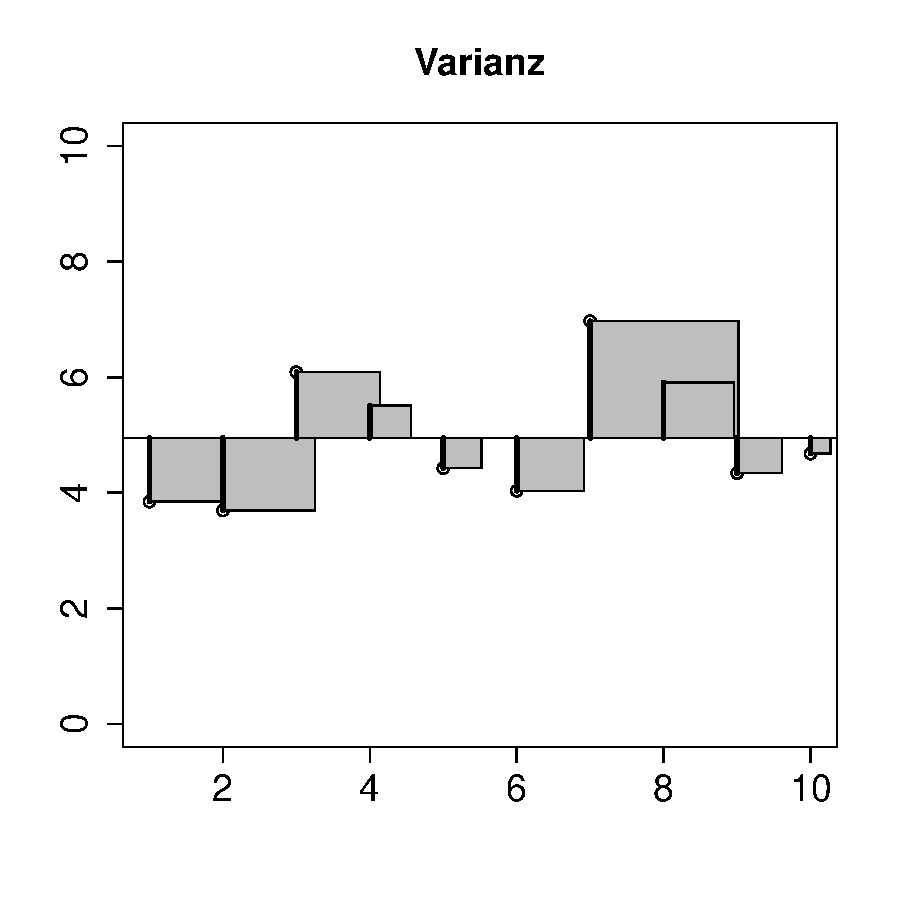
\includegraphics{begriffe-006}
\end{subfigure}
\caption{Varianz als Flächen dargestellt}
\end{figure}

\section{Standardabweichung}
Die \gls{Standardabweichung} beschreibt wie gross die die mittlere 
Abweichung ist von den einzelnen Beobachtungen (Datenpunkten) zum 
arithmetischen Mittel\footnote{Das arithmetische Mittel ist eine 
Schätzung für den
\emph{waren} Mittelwert und verändert die Formel 
(siehe Kapiel \ref{sec:varianz}).} 
derselben Beobachtungen. Die Standardabweichung ist somit gleich
der zweiten Wurzel von der Varianz der selben Beobachtungen. Die
Standardabweichung wird oft mit $\sigma$, $\sigma_x$ bzw. $s$, $s_x$ 
notiert.
\[
	\sigma_x 
	= s_x 
	= \sqrt{\sigma_{x}^2}
	= \sqrt{s_{x}^2}
	= \sqrt{\frac{1}{n-1} \cdot \left(
		\sum_{i=1}^n (x_i-\bar{x})^2 
	\right)}
\]

\paragraph{Berechnung in R}
In \lstinline{R} wird die Standardabweichung mittel \lstinline{sd()}
ermittelt. Im Folgenden ein Beispiel welches die Standardabweichung
10 zufälliger ganzer Zahlen ermittelt.
\begin{Schunk}
\begin{Sinput}
> x <- round(x=runif(n=10, min=1, max=10), digits=0)
> x
\end{Sinput}
\begin{Soutput}
 [1] 2 5 4 6 6 1 2 4 5 5
\end{Soutput}
\begin{Sinput}
> sd(x)
\end{Sinput}
\begin{Soutput}
[1] 1.763834
\end{Soutput}
\end{Schunk}
Die Standardabweichung kann auch graphisch gezeigt werden mittels
eines Plots mit \lstinline{segments()}. Dieses erlaubt es Linensegmente
zwischen \lstinline{mean()} und den Daten zu zeichnen. Die Varianz
erhält man bei der Quadrierung dieser Linien.
\begin{Schunk}
\begin{Sinput}
> x <- c(1:20)
> y <- (runif(n=20))
> plot(y)
> abline(h=mean(y))
> segments(x0=x, y0=mean(y), x1=x, y1=y, lwd=2)
\end{Sinput}
\end{Schunk}


\begin{figure}[h!]
\centering
\begin{subfigure}[b]{0.48\textwidth}
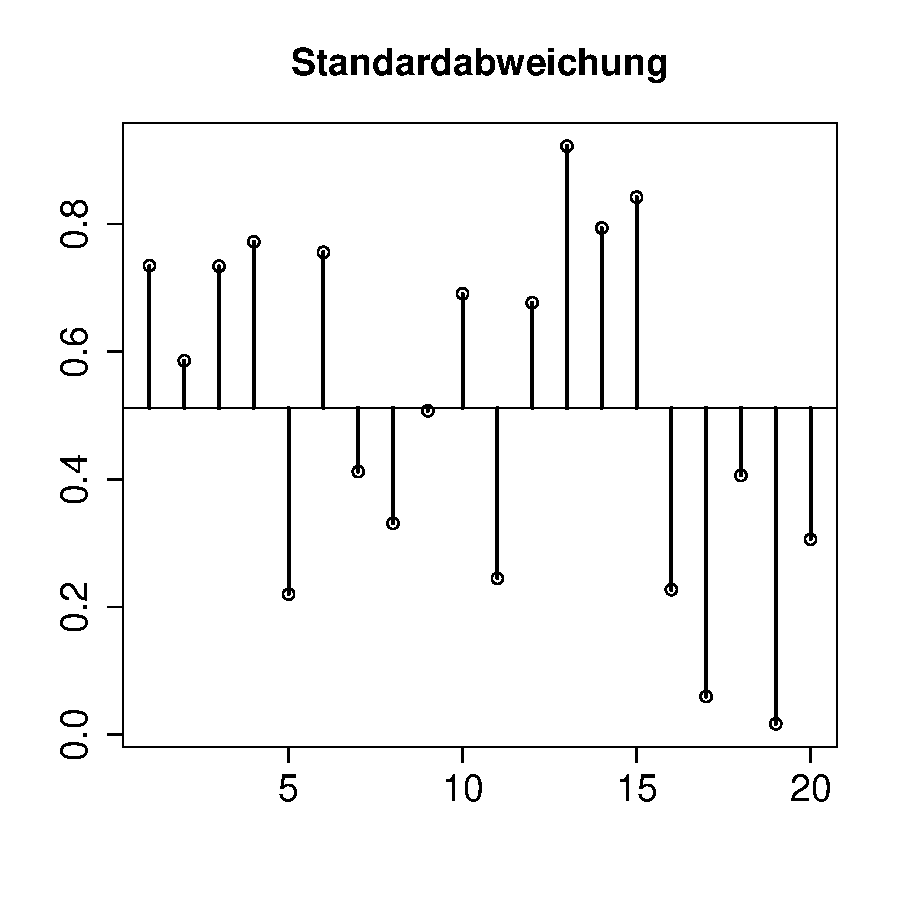
\includegraphics{begriffe-010}
\end{subfigure}
\caption{Standardabweichung (Daten zu \lstinline{mean()})}
\end{figure}

\section{Kovarianz}
Die Kovarianz (\emph{mit der Varianz}) ist ein Mass für den
Zusammenhang zweier Zufallsvariablen.
\[ \begin{array}{r c l} 
	C(X,Y) 
		&:= 
		& E((X-E(X)) \cdot (Y-E(Y))) \\
	& & \\
	s_{xy} 
		& = 
		& \displaystyle \frac{1}{n-1} \cdot \left( 
			\sum_{i=1}^n (x_i - \bar{x}) \cdot (y_i - \bar{y})
		\right)

\end{array} \]
Sie ist ein Term aus der Varianz zweier Zufallsvariablen,
denn es gilt
\[ \begin{array}{l c l} 
	V(X+Y) 
		& =
		& E(X + Y - E(X+Y))^2 \\
		& & \\
		& = 
		& V(X) + V(Y) + 2 \cdot \underbrace{
			E((X-E(X))\cdot(Y-E(Y)))}_{\text{
				Kovarianz } C(X,Y)}
\end{array} \]

Die \gls{Kovarianz} beschreibt ob sich zwei Datenreihen ähnlich 
entwickeln. Dabei gilt, dass positive Werte der Kovarianz für ein 
ähnliches Verhalten sprechen und negative dagegen. Um auch eine
Aussage über die Intensität des Zusammenhangs machen zu können,
muss die Korrelation bzw. der Korrelationskoeffizient betrachtet 
werden.

Es gibt fünf wichtige Rechenregeln für Kovarianzen.
\[ \begin{array}{l c l}
	C(X,Y) 
		& =
		& E(X \cdot Y) - (E(X) \cdot E(Y)) \\
	& & \\
	C(X,Y) 
		& =
		& C(Y,X) \\
	& & \\
	C(X,X) 
		& =
		& V(X) \\
	& & \\
	C(X,Y)
		& = 
		& C((X+a),(Y+b)) \\
	& & \\
	C(X,Y) 
		& =
		& 0 \qquad \text{falls } $X,Y$ \text{ stochastisch unabhängig} \\
\end{array} \]

\paragraph{Berechnung in R}
Die Kovarianz lässt sich in \lstinline{R} mit der Funktion 
\lstinline{cov()} ermitteln. Im Folgenden ein extremes 
Positiv-Beispiel, generiert mit je 1000 sortierten 
exponentialverteilten Zufallszahlen. 
\begin{Schunk}
\begin{Sinput}
> x <- sort(x=rexp(n=1000))
> y <- sort(x=rexp(n=1000))
> cov(x,y)
\end{Sinput}
\begin{Soutput}
[1] 1.038132
\end{Soutput}
\end{Schunk}

\section{Korrelation}
Die \gls{Korrelation} beschreibt den Zusammenhang verschiedener Variablen.
Dieser Zusammenhang kann mittels eines Koeffizienten, dem sog. 
\gls{Korrelationskoeffizient} beschrieben werden. Dieser beschreibt den
Zusammenhang mittels eines Wertes aus dem Intervall $[-1,1]$ und
hat somit auch eine Richtung.
\[ \begin{array}{r c l} 
	r(X,Y) 
		& := 
		& \displaystyle \frac{C(X,Y)}{\sqrt{V(X) \cdot V(Y)}} \\
	& & \\
	r_{xy} = \displaystyle \frac{s_{xy}}{s_x \cdot s_y}
		& = 
		& \displaystyle \frac{\sum\limits_{i=1}^n (x_i-\bar{x}) \cdot (y_i-\bar{y})}{
			\sqrt{\left(\sum\limits_{i=1}^n (x_i-\bar{x})^2\right)
			\cdot \left( \sum\limits_{i=1}^n (y_i-\bar{y})^2\right) }} \\
\end{array} \]
Mit dem Betrag und der Richtung des Korrelationskoeffizienten sind 
Grundsätzlich drei Aussagen möglich:
\[ \begin{array}{c c l r}	
	r \rightarrow +1 
		& \Rightarrow 
		& \text{Daten korrelieren positiv} 
		& \text{(\emph{je mehr, desto mehr})} \\
	r \rightarrow 0 
		& \Rightarrow 
		& \text{Daten korrelieren nicht}
		& \text{(\emph{kein Zusammenhang})} \\
	r \rightarrow -1 
		& \Rightarrow 
		& \text{Daten korrelieren negativ}
		& \text{(\emph{je mehr, desto weniger})}
\end{array} \]
\setkeys{Gin}{width=1\textwidth}
\begin{figure}[h!]
\centering
\begin{subfigure}[b]{0.3\textwidth}
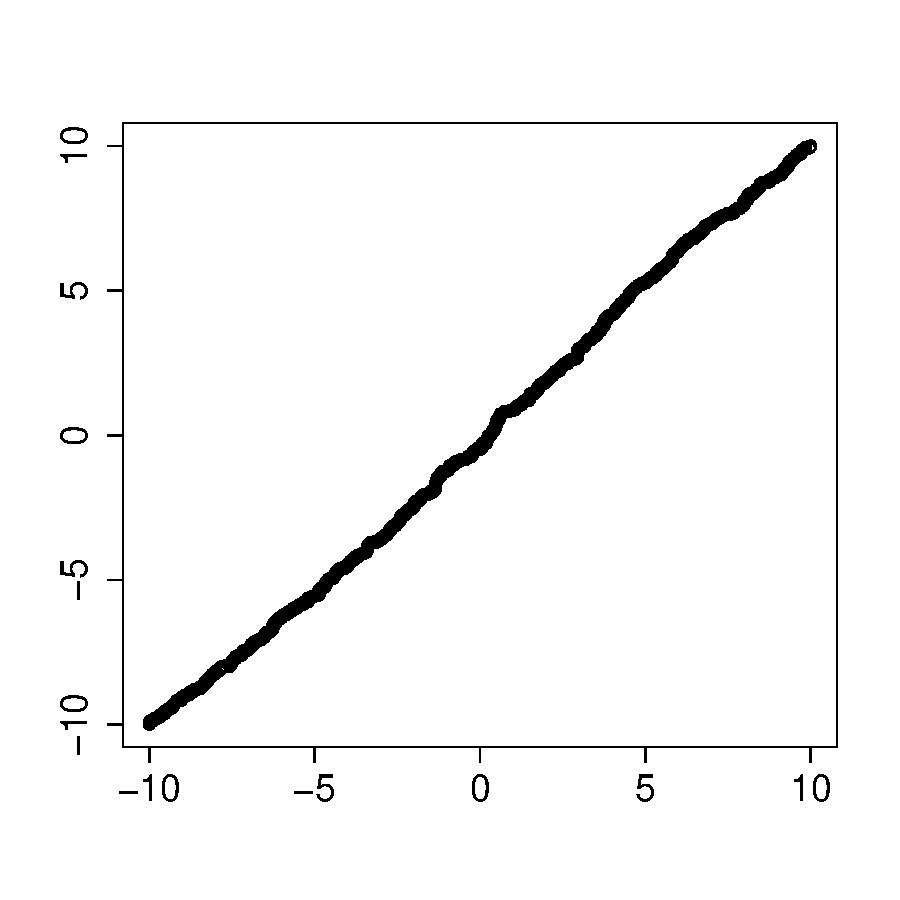
\includegraphics{begriffe-015}
\caption{$r=+1$}
\end{subfigure}
\begin{subfigure}[b]{0.3\textwidth}
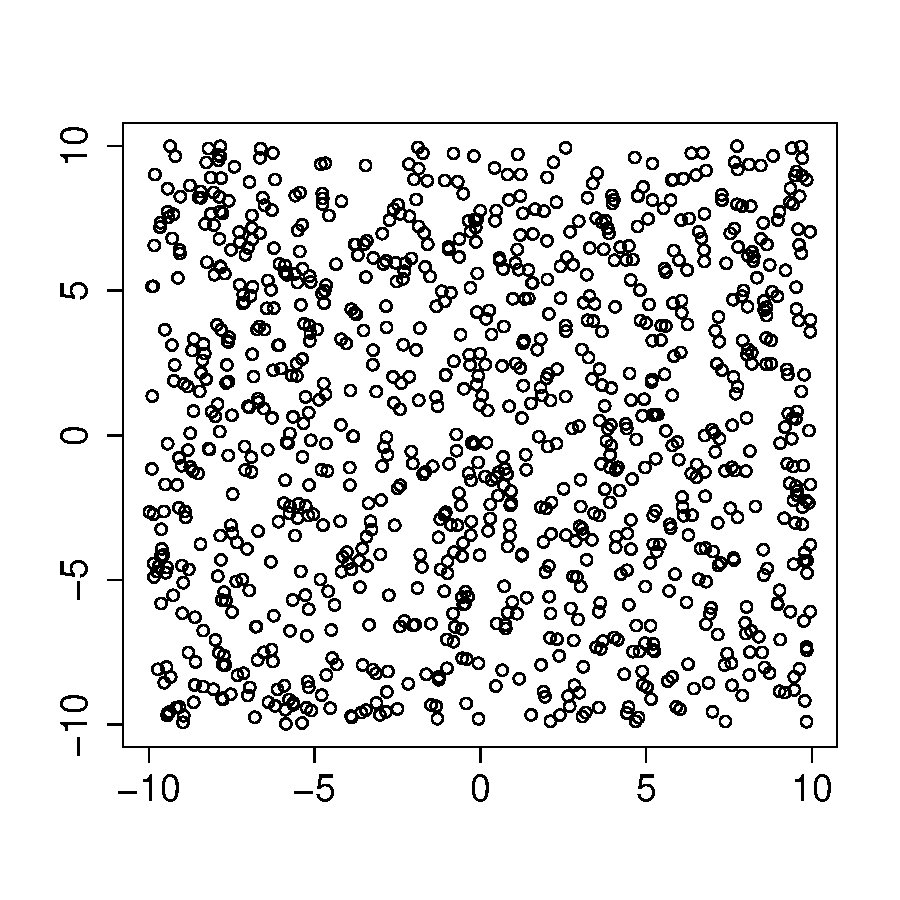
\includegraphics{begriffe-016}
\caption{$r=0$}
\end{subfigure}
\begin{subfigure}[b]{0.3\textwidth}
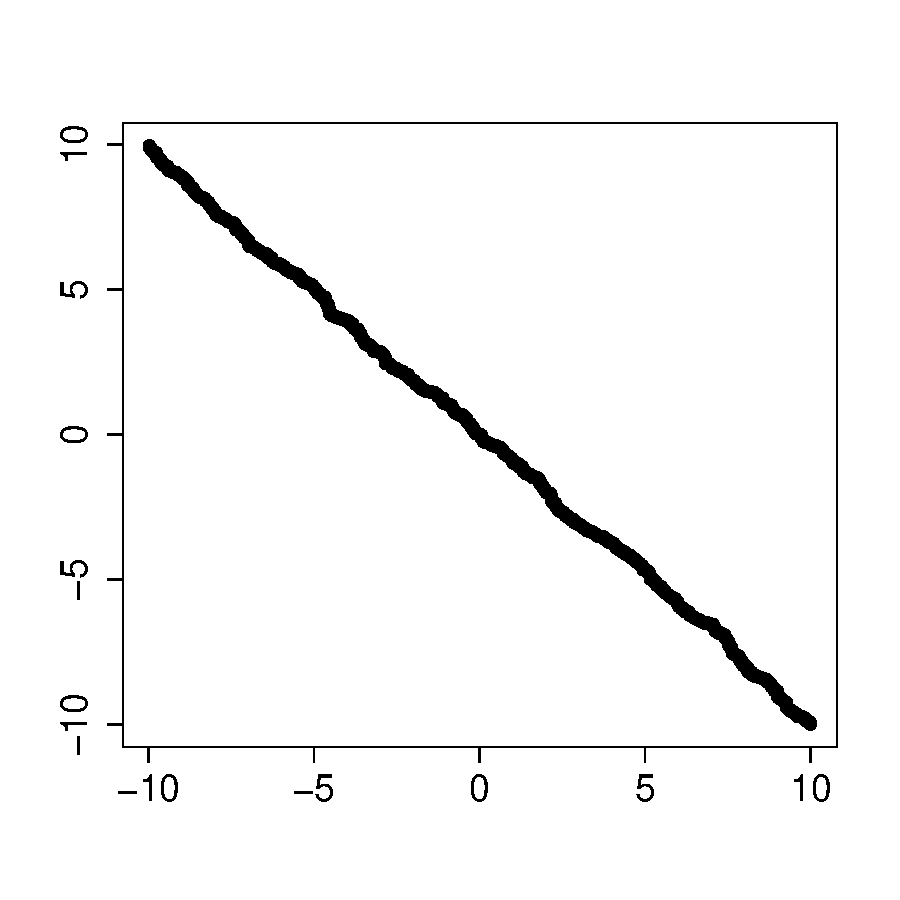
\includegraphics{begriffe-017}
\caption{$r=-1$}
\end{subfigure}
\caption{Extremwerte von Korrelationen im Vergleich.}
\label{fig:korrelation}
\end{figure}

\noindent
Bei der Analyse der Korrelation mittels solcher Plots ist Vorsicht
geboten, denn diese müssen natürlich nicht so mustergültig sein wie im 
Bild \ref{fig:korrelation} gezeigt. 
Hierzu eine kleine Merkregel: Bilden die
Daten im Plot annähernd eine Gerade mit
einer konstanten Steilheit die nicht Null ist, so korrelieren die Daten
mit annähernd $\pm1$ (Vorzeichen entsprechend der Steigung).
Ergibt sich im Plot etwas anderes als eine Gerade (etwa ein Kreis, eine
Kurve oder mehrere \emph{Wölkchen}) so ist der Korrelationskoeffizient
Null anzunehmen.

\paragraph{Berechnung in R}
In \lstinline{R} kann der Korrelationskoeffizient mit der Funktion
\lstinline{cor()} berechnet werden.

\begin{Schunk}
\begin{Sinput}
> x <- (runif(n=100)); y <- (rexp(n=100))
> cor(x,y)
\end{Sinput}
\begin{Soutput}
[1] 0.02690194
\end{Soutput}
\end{Schunk}
